

\chapter{Tobii Sono Flex}
I dette kapittelet vil den eksisterende løsningen Sono Flex bli presentert. 

\section{Tobii Sono Flex}
\label{chap:Tobii-Sono-Flex}

Programvaren som det tas utgangspunkt i heter Tobii Sono flex,  og er et systematisert symbolforråd og et verktøy for alternativ og supplerende symbolspråk. Sono flex har som mål å tilby et språk til personer som ikke enda kan lese og skrive. 

Applikasjonen fungerer som et tastatur, men istedenfor bokstaver er knappene ord med en visuell representasjon av ordet. Brukeren trykker på knappene som utgjør setningen han vil uttrykke,  programvaren vil da gjøre om setningen til tydelig tale. Systemet er spesielt utviklet for barn og unge med med sammensatte kommunikasjonsvansker som trenger et ordforråd for å videreutvikle språk- og kommunikasjonsferdigheter. 

Sono flex kan ses på som en nybegynnerpakke med en lav læringskurve som skal gjøre brukeren klar for mer avanserte systemer. Det vil si at den skal lære brukeren to ting, La brukeren bygge et vokabular og vende seg til å bruke øyesporing.


\subsection{Brukergrensesnitt}

Brukergrensesnittet til Sono flex består av to hoveddeler: en menylinje og en symboltabell. 


\subsubsection{Menylinje}

Figur \ref{fig:menylinje} viser menylinjen, som består av 5 elementer. Det hvite feltet i midten viser symbolene som brukerene har trykket på, og vil herved bli referert til som setningslisten. Symbolene som vises vil komme ut i form av tydelig tale ved å trykke på selve feltet. Knappen på venstre side av setningslisten (clear all), vil ved interaksjon tømme setningslisten. Mens knappen på høyre side vil kun fjerne det siste symbolet brukeren trykket på.


\begin{figure}[ht!]
\centering
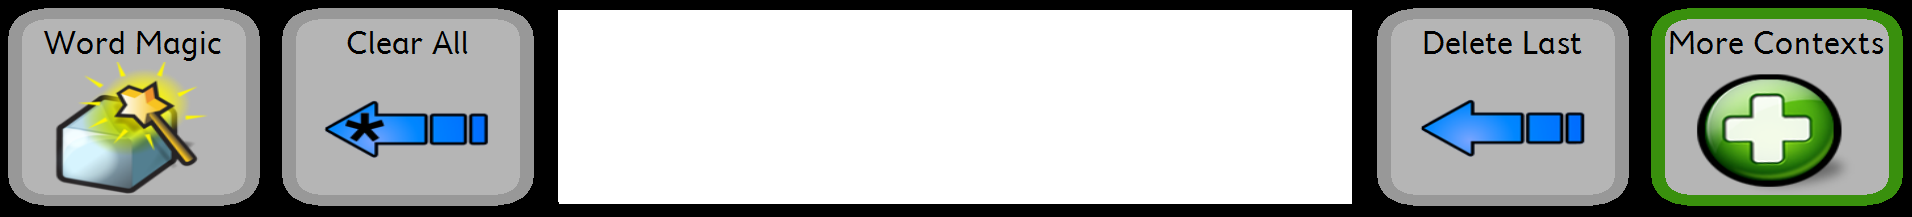
\includegraphics[width=100mm]{menylinje}
\caption{Menylinjen til programvaren Sono flex}
\label{fig:menylinje}
\end{figure}


\subsubsection{Symboltabell}
\label{subsubsec:symboltabell}

Figur \ref{fig:symbolgrid} viser applikasjonens symboltabell. Dette komponenten består av en tabell på 7 kolonner og 4 rader, noe som gir 28 celler totalt. I hver celle er det en knapp bestående av et symbol og en tekstlig beskrivelse av symbolet. Ved å trykke på knappen vil en av tre hendelser inntreffe avhengig av hvilken type symbol det er. De tre typene er ord-,kategori- og navigasjons-symbol.

Hvis knappen representerer et ord ( "jeg",  "løpe",  "kake" o.s.v. ) vil det være et ordsymbol. Ved å trykke på knappen vil symbolet og medfølgende tekst vises i setningslisten i menylinjen.

Hvis symboler har underliggende symboler som eksempelvis en ordklasse (verb,  substantiv)  eller kategori ("mat",  "frukt") vil det være et kategori symbol. Ved å trykke på knappen vil applikasjonen bytte ut de eksisterende symbolene i tabellen med ordene i ordklassen. 

Den siste typen symbol, er et navigasjonssymbol. Denne forekommer kun hvis det er for mange symboler i forhold til hvor mange det er plass til. Dersom en kategori inneholder flere symboler enn tabellstørrelsen, må symbolene fordeles over flere sider. Navigasjonssymbolet vil da være tilstede for å kunne bla mellom de ulike sidene.


\begin{figure}[ht!]
\centering
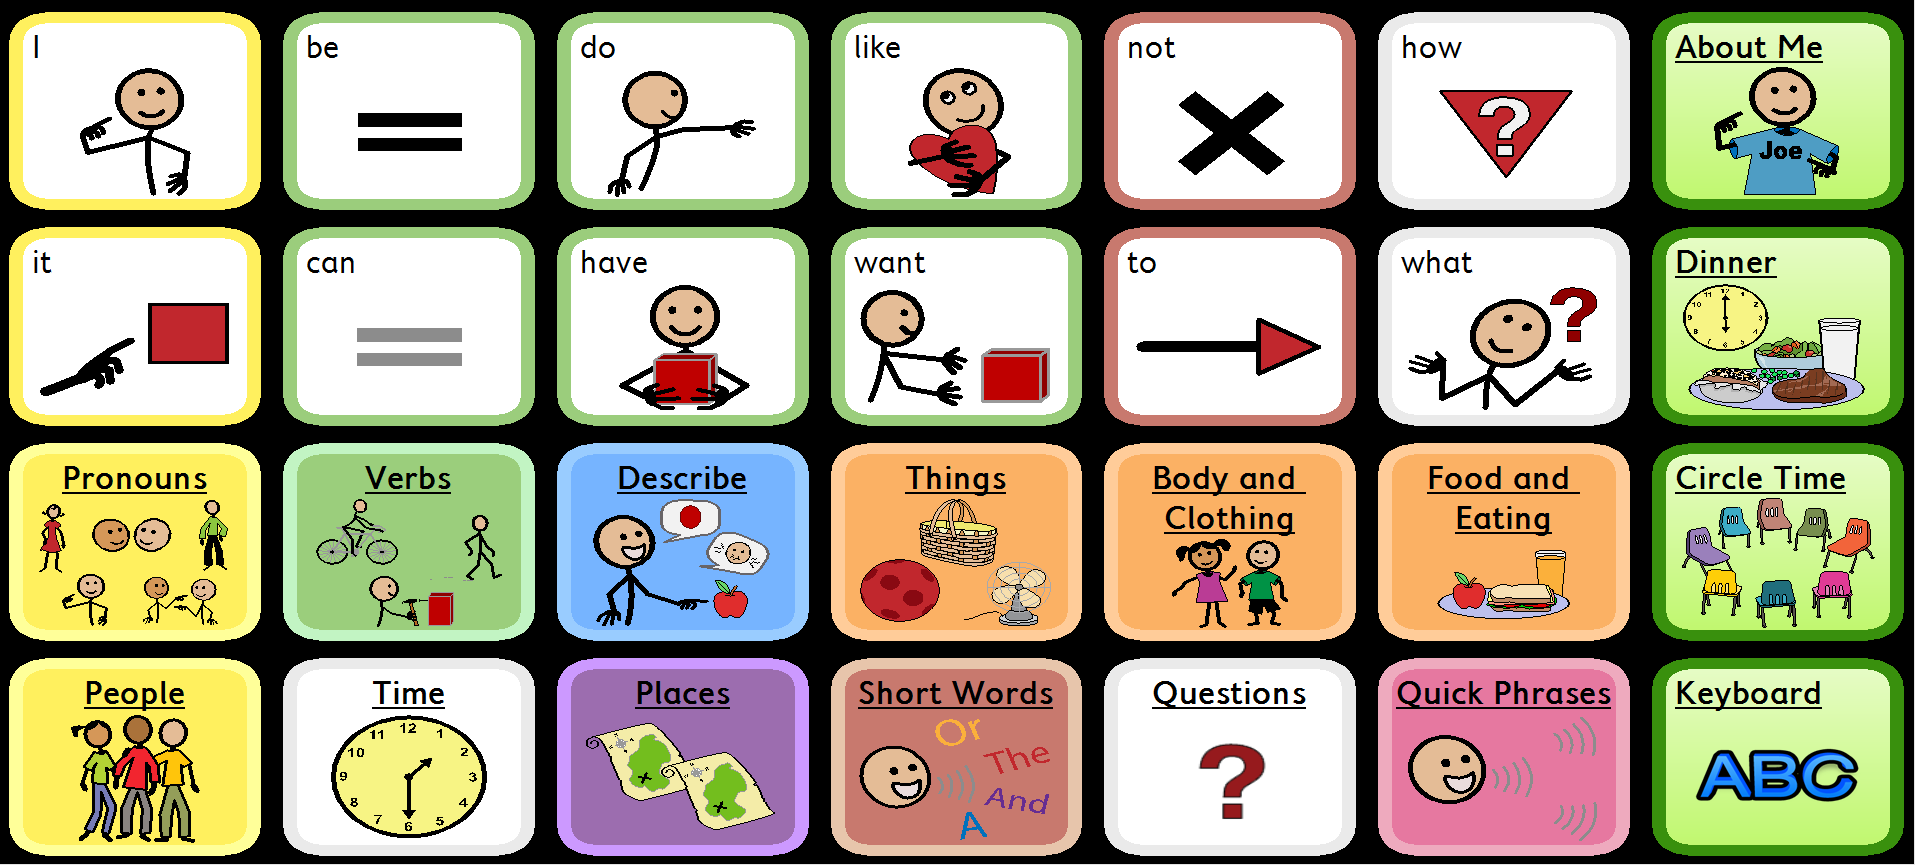
\includegraphics[width=100mm]{symbolgrid}
\caption{Symboltabellen til programvaren Sono Flex}
\label{fig:symbolgrid}
\end{figure}


\section{Kommunikasjonsform: Symboler}

De som ikke har mulighet til å bruke skrift som kommunikasjonsform kan bruke tegnsystemer. Det eksisterer tre typer tegnsystemer: håndtegn (manuelle tegn) som innebærer å bruke håndbevegelser. Materielle tegn, som vil si at en bruker fysiske objekter som brikker eller figurer. Til slutt, grafiske tegn som innebærer at en bruker symboler. 

I denne rapporten vil symbol bli brukt som kommunikasjonsform. Her representerer symboler et ord, frase, uttrykk eller setning. 

Ifølge ISAAC \cite{Tegnsystemer} er grafiske tegn brukt av mennesker med store bevegelsesvansker.
Disse menneskene har utfordringer med å lage manuelle tegn og har forståelsesvansker som følge av lærehemming. Det eksisterer flere pakker med symboler som en kan bruke for å visualisere ord \cite{GrafiskTegn}. I Sono Flex brukes en pakke kalt SymbolStix. I figur \ref{fig:katt} kan du se et eksempel på et symbol. 





\begin{figure}[ht!]
\centering
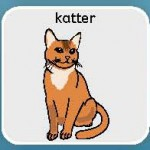
\includegraphics[width=50mm]{katt}
\caption{Symbol fra pakken SymbolStix}
\label{fig:katt}
\end{figure}

\section{Interaksjonsform: Øyesporing}

Menneske-maskin-interaksjon fungerer ved at en person gir maskinen en kommando, og maskinen svarer med en respons. For at et menneske skal kunne gi en maskin ordre, er det nødvendig at maskinen har en inputenhet som tolker beskjedene fra brukeren, slik at at datamaskinen forstår dem.  Som regel er dette tradisjonelle enheter som tastatur og mus. Det eksisterer derimot mangfoldige måter å samhandle med en maskin på.

I denne rapporten vil brukerinput bli gitt ved en øyesporingsenhet. Ved å fange opp brukerens skuepunkt med et videokamera og infrarøde lys, er det mulig for maskinen å beregne hvor på monitoren personen ser. Dette gjør interaksjon mellom dem mulig. En knapp vil for eksempel bli aktivisert ved at brukeren ser på den en viss periode. Øyesporing vil bli diskutert i neste kapittel.

\subsection{Brukerinteraksjon}

Sono Flex tilbyr to måter for brukerinteraksjon, mus og øyestyring. Mus fungerer som vanlig ved at brukeren svever med musepekeren over ønsket knapp og venstreklikker for å aktivere. Ved øyestyring må brukeren fokusere blikket på ønsket knapp en gitt tid for at applikasjonen skal tolke det som et klikk. 

Det som skjer er at med engang brukeren fokuserer blikket på en knapp vil en nedtelling starte. Figur \ref{fig:knapp-interaksjon} viser hvordan brukeren presenteres for hvor mye av nedtellingen som gjenstår.  Hvis brukeren ikke flytter blikket før nedtellingen har nådd null, tolkes dette som et klikk.
For å gi brukeren beskjed om et godkjent klikk, dannes det en rød firkant rundt knappen. 

\begin{figure}[ht!]
\centering
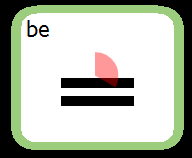
\includegraphics[width=50mm]{Knapp-interaksjon}
\caption{Skjermdump som viser hvordan nedtellingen på en knapp ser ut. Når den røde sirkelen er komplett oppfattes det som et klikk}
\label{fig:knapp-interaksjon}
\end{figure}


\section{Organisasjon og Navigasjon}

Som nevnt i seksjon \ref{subsec:navigasjon} vil et barns vokabular være såpass stort at en nødvendigvis må fordele ordene over flere sider. Sono Flex har eksempelvis 106 ord under kategorien "Ting". Med tanke på at det maksimalt er plass til 28 ord på hver side, må disse fordeles og det må finnes en måte å navigere mellom sidene på. Løsningen har blitt en svært flat struktur med et hierarki på maksimalt 2 nivåer, ergo det finnes ikke underkategorier. 

Figur \ref{fig:hieraki-ting} viser hvordan dette fungerer i praksis. Når man trykker på kategorien "ting", fylles tabellen med 27 ord som passer inn i kategorien "ting". Hvis man ikke finner ønsket ord på den første siden, navigerer man videre med knappen "neste side" og ordene i tabellen erstattes av nye ord. 


\begin{figure}[ht!]
\centering
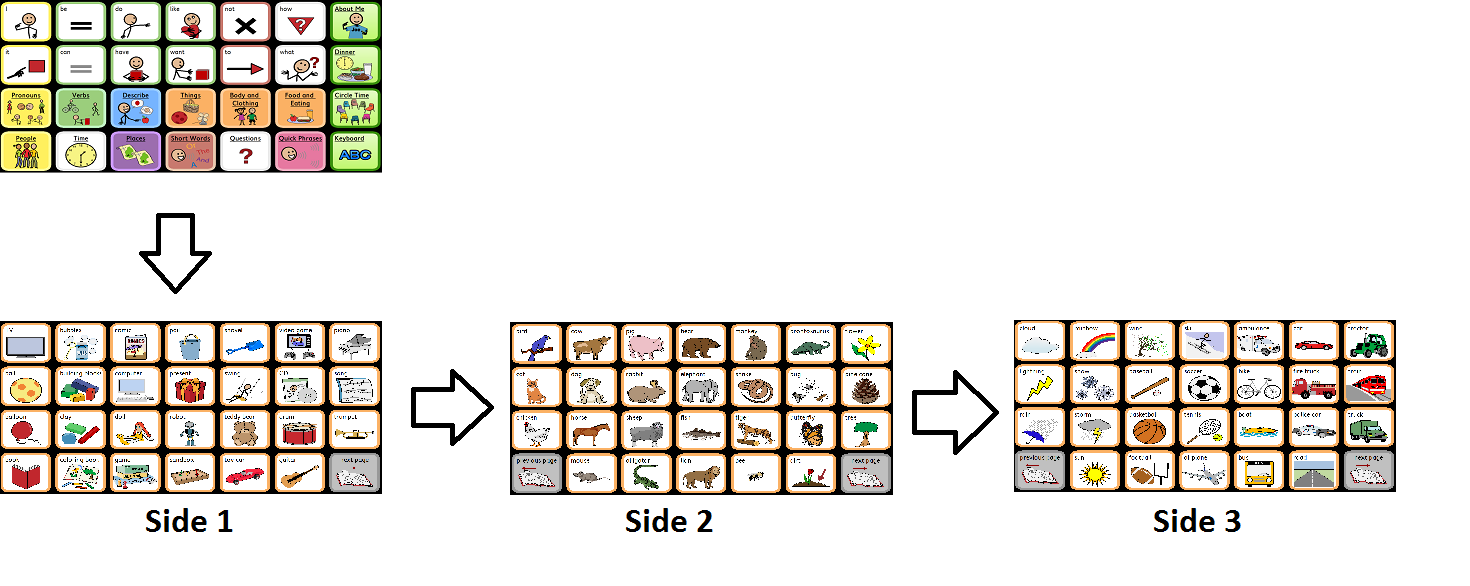
\includegraphics[width=140mm]{Symbgrid}
\caption{Skjermdump hierakiet til Sono Flex}
\label{fig:hieraki-ting}
\end{figure}
